\documentclass{standalone}
\usepackage{tikz}
\usetikzlibrary{patterns, positioning}

\begin{document}
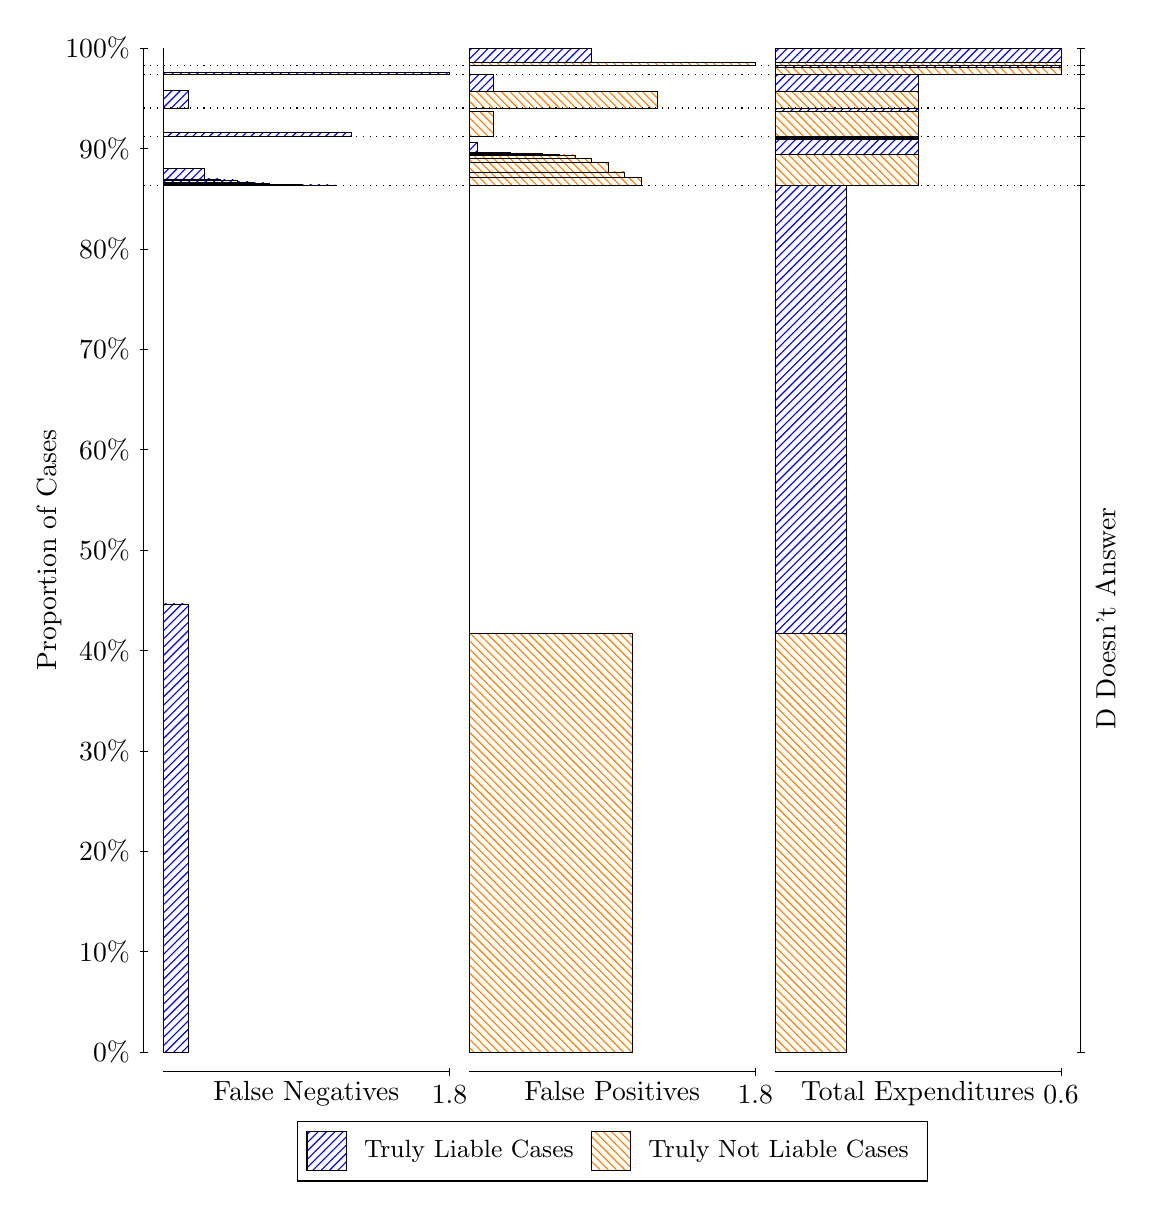
\begin{tikzpicture}
\draw[black, very thin] (1.5,1.75) -- (1.5,14.5);
\node[rotate=90, anchor=center] at (0.3, 8.125) {Proportion of Cases};
\draw[black, very thin] (1.45,1.75) -- (1.55,1.75);
\node[anchor=east] at (1.45, 1.75) {0\%};
\draw[black, very thin] (1.45,3.025) -- (1.55,3.025);
\node[anchor=east] at (1.45, 3.025) {10\%};
\draw[black, very thin] (1.45,4.3) -- (1.55,4.3);
\node[anchor=east] at (1.45, 4.3) {20\%};
\draw[black, very thin] (1.45,5.575) -- (1.55,5.575);
\node[anchor=east] at (1.45, 5.575) {30\%};
\draw[black, very thin] (1.45,6.85) -- (1.55,6.85);
\node[anchor=east] at (1.45, 6.85) {40\%};
\draw[black, very thin] (1.45,8.125) -- (1.55,8.125);
\node[anchor=east] at (1.45, 8.125) {50\%};
\draw[black, very thin] (1.45,9.4) -- (1.55,9.4);
\node[anchor=east] at (1.45, 9.4) {60\%};
\draw[black, very thin] (1.45,10.675) -- (1.55,10.675);
\node[anchor=east] at (1.45, 10.675) {70\%};
\draw[black, very thin] (1.45,11.95) -- (1.55,11.95);
\node[anchor=east] at (1.45, 11.95) {80\%};
\draw[black, very thin] (1.45,13.225) -- (1.55,13.225);
\node[anchor=east] at (1.45, 13.225) {90\%};
\draw[black, very thin] (1.45,14.5) -- (1.55,14.5);
\node[anchor=east] at (1.45, 14.5) {100\%};

\draw[black, very thin] (13.4,1.75) -- (13.4,14.5);
\draw[black, very thin] (13.35,1.75) -- (13.45,1.75);
\node[anchor=west] at (13.35, 1.75) {};
\draw[black, very thin] (13.35,12.759) -- (13.45,12.759);
\node[anchor=west] at (13.35, 12.759) {};
\draw[black, very thin] (13.35,13.379) -- (13.45,13.379);
\node[anchor=west] at (13.35, 13.379) {};
\draw[black, very thin] (13.35,13.738) -- (13.45,13.738);
\node[anchor=west] at (13.35, 13.738) {};
\draw[black, very thin] (13.35,14.168) -- (13.45,14.168);
\node[anchor=west] at (13.35, 14.168) {};
\draw[black, very thin] (13.35,14.279) -- (13.45,14.279);
\node[anchor=west] at (13.35, 14.279) {};
\draw[black, very thin] (13.35,14.5) -- (13.45,14.5);
\node[anchor=west] at (13.35, 14.5) {};

\draw[black, very thin, pattern color=blue, pattern=north east lines] (1.75,1.75) rectangle (2.0614,7.44);
\draw[black, very thin, pattern color=orange, pattern=north west lines] (1.75,7.44) rectangle (1.75,12.759);
\draw[black, very thin, pattern color=blue, pattern=north east lines] (1.75,12.759) rectangle (3.93,12.761);
\draw[black, very thin, pattern color=blue, pattern=north east lines] (1.75,12.761) rectangle (3.7224,12.763);
\draw[black, very thin, pattern color=blue, pattern=north east lines] (1.75,12.763) rectangle (3.5148,12.767);
\draw[black, very thin, pattern color=blue, pattern=north east lines] (1.75,12.767) rectangle (3.3071,12.771);
\draw[black, very thin, pattern color=blue, pattern=north east lines] (1.75,12.771) rectangle (3.0995,12.786);
\draw[black, very thin, pattern color=blue, pattern=north east lines] (1.75,12.786) rectangle (2.8919,12.8);
\draw[black, very thin, pattern color=blue, pattern=north east lines] (1.75,12.8) rectangle (2.6843,12.824);
\draw[black, very thin, pattern color=blue, pattern=north east lines] (1.75,12.824) rectangle (2.4767,12.838);
\draw[black, very thin, pattern color=blue, pattern=north east lines] (1.75,12.838) rectangle (2.269,12.967);
\draw[black, very thin, pattern color=orange, pattern=north west lines] (1.75,12.967) rectangle (1.75,13.379);
\draw[black, very thin, pattern color=blue, pattern=north east lines] (1.75,13.379) rectangle (4.1376,13.426);
\draw[black, very thin, pattern color=orange, pattern=north west lines] (1.75,13.426) rectangle (1.75,13.738);
\draw[black, very thin, pattern color=blue, pattern=north east lines] (1.75,13.738) rectangle (2.0614,13.958);
\draw[black, very thin, pattern color=orange, pattern=north west lines] (1.75,13.958) rectangle (1.75,14.168);
\draw[black, very thin, pattern color=blue, pattern=north east lines] (1.75,14.168) rectangle (5.3833,14.194);
\draw[black, very thin, pattern color=orange, pattern=north west lines] (1.75,14.194) rectangle (1.75,14.279);
\draw[black, very thin, pattern color=orange, pattern=north west lines] (1.75,14.279) rectangle (1.75,14.317);
\draw[black, very thin, pattern color=blue, pattern=north east lines] (1.75,14.317) rectangle (1.75,14.5);
\draw[black, very thin, pattern color=orange, pattern=north west lines] (5.6333,1.75) rectangle (7.7095,7.0686);
\draw[black, very thin, pattern color=blue, pattern=north east lines] (5.6333,7.0686) rectangle (5.6333,12.759);
\draw[black, very thin, pattern color=orange, pattern=north west lines] (5.6333,12.759) rectangle (7.8133,12.86);
\draw[black, very thin, pattern color=orange, pattern=north west lines] (5.6333,12.86) rectangle (7.6057,12.927);
\draw[black, very thin, pattern color=orange, pattern=north west lines] (5.6333,12.927) rectangle (7.3981,13.044);
\draw[black, very thin, pattern color=orange, pattern=north west lines] (5.6333,13.044) rectangle (7.1905,13.096);
\draw[black, very thin, pattern color=orange, pattern=north west lines] (5.6333,13.096) rectangle (6.9829,13.144);
\draw[black, very thin, pattern color=orange, pattern=north west lines] (5.6333,13.144) rectangle (6.7752,13.148);
\draw[black, very thin, pattern color=orange, pattern=north west lines] (5.6333,13.148) rectangle (6.7752,13.153);
\draw[black, very thin, pattern color=orange, pattern=north west lines] (5.6333,13.153) rectangle (6.5676,13.162);
\draw[black, very thin, pattern color=orange, pattern=north west lines] (5.6333,13.162) rectangle (6.36,13.166);
\draw[black, very thin, pattern color=orange, pattern=north west lines] (5.6333,13.166) rectangle (6.1524,13.17);
\draw[black, very thin, pattern color=blue, pattern=north east lines] (5.6333,13.17) rectangle (5.7371,13.3);
\draw[black, very thin, pattern color=blue, pattern=north east lines] (5.6333,13.3) rectangle (5.6333,13.379);
\draw[black, very thin, pattern color=orange, pattern=north west lines] (5.6333,13.379) rectangle (5.9448,13.691);
\draw[black, very thin, pattern color=blue, pattern=north east lines] (5.6333,13.691) rectangle (5.6333,13.738);
\draw[black, very thin, pattern color=orange, pattern=north west lines] (5.6333,13.738) rectangle (8.021,13.947);
\draw[black, very thin, pattern color=blue, pattern=north east lines] (5.6333,13.947) rectangle (5.9448,14.168);
\draw[black, very thin, pattern color=orange, pattern=north west lines] (5.6333,14.168) rectangle (5.6333,14.252);
\draw[black, very thin, pattern color=blue, pattern=north east lines] (5.6333,14.252) rectangle (5.6333,14.279);
\draw[black, very thin, pattern color=orange, pattern=north west lines] (5.6333,14.279) rectangle (9.2667,14.317);
\draw[black, very thin, pattern color=blue, pattern=north east lines] (5.6333,14.317) rectangle (7.1905,14.5);
\draw[black, very thin, pattern color=orange, pattern=north west lines] (9.5167,1.75) rectangle (10.425,7.0686);
\draw[black, very thin, pattern color=blue, pattern=north east lines] (9.5167,7.0686) rectangle (10.425,12.759);
\draw[black, very thin, pattern color=orange, pattern=north west lines] (9.5167,12.759) rectangle (11.333,13.148);
\draw[black, very thin, pattern color=blue, pattern=north east lines] (9.5167,13.148) rectangle (11.333,13.346);
\draw[black, very thin, pattern color=orange, pattern=north west lines] (9.5167,13.346) rectangle (11.333,13.351);
\draw[black, very thin, pattern color=blue, pattern=north east lines] (9.5167,13.351) rectangle (11.333,13.353);
\draw[black, very thin, pattern color=orange, pattern=north west lines] (9.5167,13.353) rectangle (11.333,13.371);
\draw[black, very thin, pattern color=blue, pattern=north east lines] (9.5167,13.371) rectangle (11.333,13.379);
\draw[black, very thin, pattern color=orange, pattern=north west lines] (9.5167,13.379) rectangle (11.333,13.691);
\draw[black, very thin, pattern color=blue, pattern=north east lines] (9.5167,13.691) rectangle (11.333,13.738);
\draw[black, very thin, pattern color=orange, pattern=north west lines] (9.5167,13.738) rectangle (11.333,13.947);
\draw[black, very thin, pattern color=blue, pattern=north east lines] (9.5167,13.947) rectangle (11.333,14.168);
\draw[black, very thin, pattern color=orange, pattern=north west lines] (9.5167,14.168) rectangle (13.15,14.252);
\draw[black, very thin, pattern color=blue, pattern=north east lines] (9.5167,14.252) rectangle (13.15,14.279);
\draw[black, very thin, pattern color=orange, pattern=north west lines] (9.5167,14.279) rectangle (13.15,14.317);
\draw[black, very thin, pattern color=blue, pattern=north east lines] (9.5167,14.317) rectangle (13.15,14.5);
\draw[black, dotted] (1.5,12.759) -- (13.4,12.759);
\draw[black, dotted] (1.5,13.379) -- (13.4,13.379);
\draw[black, dotted] (1.5,13.738) -- (13.4,13.738);
\draw[black, dotted] (1.5,14.168) -- (13.4,14.168);
\draw[black, dotted] (1.5,14.279) -- (13.4,14.279);
\draw[black, very thin] (1.75,1.5) -- (5.3833,1.5);
\node[anchor=north] at (3.5667, 1.5) {False Negatives};
\draw[black, very thin] (5.3833,1.45) -- (5.3833,1.55);
\node[anchor=north] at (5.3833, 1.45) {1.8};

\draw[black, very thin] (5.6333,1.5) -- (9.2667,1.5);
\node[anchor=north] at (7.45, 1.5) {False Positives};
\draw[black, very thin] (9.2667,1.45) -- (9.2667,1.55);
\node[anchor=north] at (9.2667, 1.45) {1.8};

\draw[black, very thin] (9.5167,1.5) -- (13.15,1.5);
\node[anchor=north] at (11.333, 1.5) {Total Expenditures};
\draw[black, very thin] (13.15,1.45) -- (13.15,1.55);
\node[anchor=north] at (13.15, 1.45) {0.6};

\node[black, centered, rotate=90] at (13.72, 7.2543) {D Doesn't Answer};






\draw (7.449999999999999,1.5) node[draw=none] (baseCoordinate) {};
\begin{scope}[align=center]
        \matrix[scale=0.5, draw=black, below=0.5cm of baseCoordinate, nodes={draw}, column sep=0.1cm]{
            \node[rectangle, draw, minimum width=0.5cm, minimum height=0.5cm, pattern=north east lines, pattern color=blue] {}; &
            \node[draw=none, font=\small] (B) {Truly Liable Cases}; &
            \node[rectangle, draw, minimum width=0.5cm, minimum height=0.5cm, pattern=north west lines, pattern color=orange] {}; &
            \node[draw=none, font=\small] (B) {Truly Not Liable Cases}; \\
            };
\end{scope}

\end{tikzpicture}
\end{document}